\chapter{Introduction}

In this thesis, we will develop the theory of minimal surfaces from the point of view of geometric measure theory. As motivation, we will, in the introduction, quickly look at minimal surfaces in $3$-dimensional space. We shall see what a minimal surface is, and see some examples.

In the main part of the thesis, we will then try and generalize the idea of a minimal surface. We shall take the procedure and tools from the 3-dimensional case, and generalize them to higher dimensions, and a broader class of surfaces. To that end the first few chapters are going to lay the groundwork, with the basics of geometric measure theory, and then the last chapters will introduce varifolds, which will be our generalized surfaces. We will define the analogous notion of a "minimal" varifold, and we shall show some regularity results about varifolds ultimately seeking to show Allard's regularity theorem.

This thesis follows various sources, but will try and give a gentler and easier introduction to the topic than for instance the canonical textbook in the field, \cite{simon2014introduction}, which is a bit difficult to read for those uninitiated. Hopefully this thesis will help in that aspect, by clearing up some ambiguities, and fleshing out important details where needed.

The introduction takes roots in the examples from \cite{holopainen15}, and then tries to give a quick look at the 3-dimensional minimal surfaces based on those.

The following chapter, on the Hausdorff measure and area formulae, are meant as preliminary chapters, and will introduce basic but very important concepts to be able to discuss generalized minimal surfaces, especially the Hausdorff measure will be present a.e. in the thesis. This chapters takes inspiration from \cite{holopainen16}.

The following chapters are then going to build up to varifolds and then show various results, culminating in Allard's regularity theorem. See \cite{holopainen16}, \cite{simon2014introduction} and \cite{DeL12} amongst others.

But before all that...

\section{Minimal surfaces in $\R^3$}
We are interested in finding surfaces, bounded by closed curves, which minimizes their area. I.e. of all the surfaces spanning a given boundary, we seek the surface(s) with the least area of those.

Minimal surface theory lies at the intersection of many different fields of mathematics. This becomes clear when one sees the many different equivalent definitions of a minimal surface. Indeed a surface in $\R^3$ is said to be minimal if it satisfies one of the following equivalent definitions.
\begin{enumerate}
    \item \emph{Local area-minimising definition}. A surface $S \subseteq \R^3$ is minimal if around each point $p \in S$ there is a neighborhood which has minimal area with respect to its boundary. \cite{holopainen15}
    
    This local definition is actually not equivalent to the others, as there might be surfaces with smaller area, but with the same boundary.
    \item \emph{Variational definition}. A surface $S \subseteq \R^3$ is minimal if and only if it a critical point of the area functional for all compactly supported variations.
    
    This definition shows that minimal surfaces are analogous to geodesics. \cite{holopainen15}
    
    \item \emph{Mean Curvature definition}. A surface $S \subseteq \R^3$ is minimal if and only if its mean curvature is zero. \cite{holopainen15}
    
    \item \emph{Gauss map definition}: A surface $M \subseteq R^3$ is minimal if and only if its stereographically projected Gauss map $g: M \to C \cup \{ \infty \}$ is meromorphic with respect to the underlying Riemann surface structure, and $M$ is not a piece of a sphere.\cite{holopainen15}
\end{enumerate}
See \cite{holopainen15} for even more equivalent definitions.

We shall be most interested in the third definition when we try and generalize minimal surfaces. However for the 3-dimensional case, we shall also make use of the second definition.

Let us briefly discuss the variational definition of a minimal surface in $\R^3$. This brief discussion will provide a scaffold on which to build our more general theory of minimal surfaces, as the tools and process shown here will be generalizable to higher dimensions, and a wider class of surfaces.

Let $U \subseteq \R^3$ be open and bounded, let $u:U \to \R$ be $C^2$ and let
\[
    \Gamma_u:=\{(x,y,u(x,y)) \mid (x,y) \in U\} \subseteq \R^3
\]
be the graph of $u$.
Then $\Gamma_u$ is a $2$-dimensional submanifold of $\R^3$, which for every $p=(x,y,u(x,y))\in \Gamma_u$ has the tangent space $T_p\Gamma_u$ spanned by the vectors $(1,0,u_x)$ and $(0,1,u_y)$, where $u_x$ and $u_y$ denote the partial derivatives of $u$ with respect to $x$ and $y$ respectively.

We are interested in the area of $\Gamma_u$ as a submanifold, in order to be able to determine if it has least area. Now, the area of the graph $\Gamma_u$ is given by
\begin{align}
    \Area(\Gamma_u) &= \int_U \left| (1,0,u_x) \times (0,1,u_y) \right|\, d\lambda \nonumber \\
    &= \int_U \sqrt{1+|\nabla u|^2}\, d\lambda. \label{eq: 3 area formula}
\end{align}
Where $\lambda$ is the 1-dimensional Lebesgue measure.
Now, we are going to perturb the graph by a $C^2$-map, that is, we consider $u'=u+t\eta$ for some $\eta \in C^2$ and small $t$. However, $u$ is supposed minimal, so the area of $u'$ should be minimized when $s=0$. That is, $u$ should be a critical point when varying $t$.

So let $\eta \in C_c^2(U)$.
Then for every $t \in \R$, $\Gamma_u$ and $\Gamma_{u+t\eta}$ have the same boundary $\partial \Gamma_u:=\{(x,y,u(x,y)) \mid (x,y) \in \partial U\}$ and
\[
    \Area(\Gamma_{u+t\eta}) = \int_U \sqrt{1 + |\nabla u + t\nabla \eta|^2}\, d\lambda.
\]
We now differentiate with respect to $t$ and use Greens formula to get
\begin{align*}
    \frac{d}{dt}\Area(\Gamma_{u+t\eta})|_{t=0} &= \frac{d}{dt} \int_U \sqrt{1 + |\nabla u + t\nabla \eta|^2}|_{t=0}\, d\lambda \\
    &= \int_U \frac{d}{dt} \sqrt{1 + |\nabla u + t\nabla \eta|^2}|_{t=0}\, d\lambda \\
    &= \int_U \frac{1}{2\sqrt{1+|\nabla u|^2}}\frac{d}{dt}\angles{\nabla(u+t\eta), \nabla(u+t\eta)}|_{t=0}\, d\lambda \\
    &= \int_U \frac{\angles{\nabla u, \nabla\eta}}{\sqrt{1+|\nabla u|^2}}\, d\lambda \\
    &= -\int_U \eta \Div\paren{\frac{\nabla u}{\sqrt{1+|\nabla u|^2}}}\, d\lambda.
\end{align*}
We say that $u$ is a critical point (of the area functional) if this above differential is zero at $t=0$. If the differential is zero, then $\eta$ would vanish in the last equation for all $\eta \in C_c^2(U)$, so $u$ is a critical point if and only if
\[
    \Div\paren{\frac{\nabla u}{\sqrt{1+|\nabla u|^2}}} = 0.
\]
By the variational definition of a minimal surface, we thus see that a graph $\Gamma_u$ is a minimal surface if and only if $u$ is a critical point of the area functional.


Now, Let $u$ be a critical point of the area functional, and $\Gamma_u \subseteq U \times \R$ be the graph of $u$. We want to show that $\Gamma_u$ in fact minimizes area among all surfaces on the cylinder $U \times \R$ with the same boundary, $\partial \Gamma_u$.

To do that, we define $N$ to be the unit vector
\[
    N := \frac{(1,0,u_x) \times (0,1,u_y)}{|(1,0,u_x) \times (0,1,u_y)|} = \frac{(1,0,u_x) \times (0,1,u_y)}{\sqrt{1+|\nabla u|^2}}.
\]
By the nature of the cross product, $N$ is orthogonal to both $(1,0,u_x)$ and $(0,1,u_y)$ and it is therefore the upward pointing unit normal to $\Gamma_u$.

We then define a 2-form $\omega:(U \times \R)^2 \to \R$ by
\[
    \omega(X,Y) = \det(X,Y,N) := \det\begin{pmatrix}
    | & | & | \\
    X & Y & N \\
    | & | & |
    \end{pmatrix}
\]
for $X,Y \in \R^3$. Note that $\omega$ is really just contraction by $N$ of the standard volume formula $\tilde\omega=dx \wedge dy \wedge dz$.
Therefore $\omega$ is the volume (or area) form of $\Gamma_u$.

Now with
\begin{align*}
    a &:= \omega\paren{\frac{\partial}{\partial x}, \frac{\partial}{\partial y}} = \frac{1}{\sqrt{1+|\nabla u|^2}} \\
    b &:= \omega\paren{\frac{\partial}{\partial x}, \frac{\partial}{\partial z}} = \frac{u_y}{\sqrt{1+|\nabla u|^2}} \\
    c &:= \omega\paren{\frac{\partial}{\partial y}, \frac{\partial}{\partial z}} = \frac{-u_x}{\sqrt{1+|\nabla u|^2}} \\
\end{align*}
we have that
\begin{align*}
    \omega &=a\, dx\wedge dy + b\, dx\wedge dz + c\, dy\wedge dz \\
    &= \frac{dx\wedge dy - u_x\, dy\wedge dz - u_y\, dz\wedge dy}{\sqrt{1+|\nabla u|^2}}.
\end{align*}
Moreover, since $u$ is a critical point of the area functional
\[
    d\omega = \left[ \frac{\partial}{\partial x} \paren{\frac{-u_x}{\sqrt{1+|\nabla u|^2}}} + \frac{\partial}{\partial y}\paren{\frac{-u_y}{\sqrt{1+|\nabla u|^2}}} \right] dx \wedge dy \wedge dz = 0.
\]
Hence $d\omega$ is a closed 2-form in the cylinder $U \times \R$, so if $\Sigma$ is another smooth surface in $U \times \R$ with $\partial \Sigma = \partial \Gamma_u$, then $\Sigma$ and $\Gamma_u$ enclose an open set $O \subseteq \R^3$ in which $d\omega=0$. Now, $O$ may not be connected, and have several components, but by applying Stokes theorem in each of these components we see that
\[
    \int_{\Gamma_u}\omega = \int_{\Sigma}\omega.
\]
On the other hand, by definition, $|\omega(X,Y)| = |\det(X,Y,N)|$ is the volume of the polyhedron spanned by $X,Y$ and $N$ so in particular
\[
    |\omega(X,Y)| \le 1
\]
for all unit vectors $X,Y\in \R^3$. Equality holds above when $X,Y,N$ are orthonormal. This implies that
\[
    \Area(\Gamma_u) = \int_{\Gamma_u}\omega = \int_{\Sigma} \le \Area(\Sigma)
\]
which implies that $\Gamma_u$ minimizes area.
\begin{example}
Examples of minimal surfaces:
\begin{enumerate}
\item The plane $u(x,y)=0$, which is clearly a critical point of the area functional.
\item The helicoid (see \cref{fig: helicoid}) $u(x,y)=\arctan(y/x)$. Indeed
\[
    u_x = \frac{-y}{x^2+y^2}, \quad \text{and} \quad u_y=\frac{x}{x^2+y^2}
\]
Hence
\[
    v(x,y):=\sqrt{1+|\nabla u|^2} = \sqrt{\frac{1+x^2+y^2}{x^2+y^2}}
\]
and we get that $v_x(y,x)=(4x^3+4xy^2+2x)/v(x,y)$ and $v_y(x,y)=v_x(y,x)$, therefore
\[
    \Div\paren{\frac{\nabla u}{\sqrt{1+|\nabla u|^2}}} = \frac{yv_x-xv_y}{v(x,y)^2} = 0
\]
So the helicoid is a minimal surface.

One could also have found the mean curvature of the helicoid, and found that it is zero as well. Indeed
the helecoid can be parametrized as
\[
    r(s,t) = (s\cos(t),s\sin(t),t)
\]
for $s,t \in \R$.

We find the partial derivatives up to order two, and get
\begin{align*}
    \frac{\partial r}{\partial u} &= (\cos(v),\sin(v),0), \\
    \frac{\partial r}{\partial v} &= (-u\sin(v), u\cos(v),1) \\
    \frac{\partial^2 r}{\partial u^2} &= (0,0,0),\\ \frac{\partial^2 r}{\partial u \partial v} &= (-\sin(v),\cos(v),0) \\
    \frac{\partial^2 r}{\partial v^2} &= (-u\cos(v),-u\sin(v),0) \\
\end{align*}
We find the unit normal
\begin{align*}
    N = \frac{\frac{\partial r}{\partial u} \times \frac{\partial t}{\partial v}}{\left| \frac{\partial r}{\partial u} \times \frac{\partial t}{\partial v} \right|} = \frac{1}{\sqrt{1+u^2}}(\sin(v),-\cos(v),u)
\end{align*}
Then the first and second fundamental forms are
\begin{align*}
    I(u,v) = \begin{pmatrix}
    1 & 0 \\
    0 & 1+u^2
    \end{pmatrix}, \quad \text{ and } \quad II(u,v) = \frac{1}{\sqrt{1+u^2}}\begin{pmatrix}
    0 & 1 \\
    1 & 0
    \end{pmatrix}
\end{align*}
And then the principal curvatures are the solutions to the characteristic equation
\[
    \det(II(u,v)-\kappa I(u,v)) = \kappa^2(1+u^2)-\frac{1}{\sqrt{1+u^2}}=0
\]
which means that the principal curvatures are $\pm 1/(1+u^2)$. Since the mean curvature is the average of the principal curvatures, we see that the mean curvature of the helicoid is $0$.
\item The catenoid (see \cref{fig: catenoid}) $u(x,y)=\cosh^{-1}(\sqrt{x^2+y^2})$. By going through the same steps as above, one sees that the catenoid is indeed a minimal surface.
\item Enneper's surface (see \cref{fig: enneper}) which is parametrized by
\[
    (s,t) \mapsto \paren{s-\frac{s^3}{3}+st^2, -t-s^2t+\frac{t^3}{3}, s^2-t^2}
\]
for $s,t \in \R$.
\end{enumerate}

\begin{figure}
    \centering
    \begin{subfigure}[b]{0.3\textwidth}
        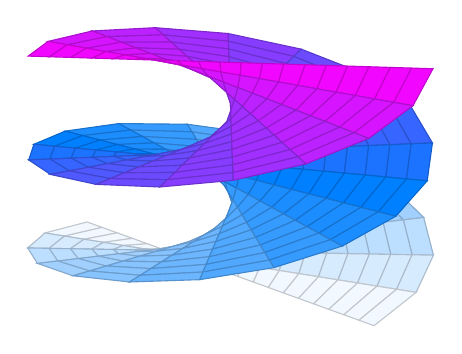
\begin{tikzpicture}
          \begin{axis}[
          hide axis
          ]
             \addplot3[
                 surf,
                 colormap/cool,
                 samples=20,
                 domain=-200:200,
                 y domain=-10:10,
                 z buffer=sort
               ]
               ( {y*cos(x)}, 
                 {y*sin(x)}, 
                 {x}
               );
          \end{axis}
          
        \end{tikzpicture}
        \caption{A Helicoid}
        \label{fig: helicoid}
    \end{subfigure}
    ~ 
    \begin{subfigure}[b]{0.3\textwidth}
        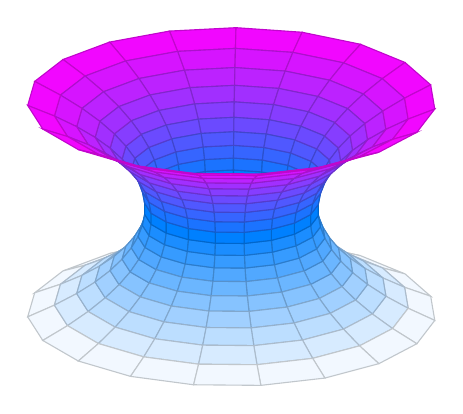
\begin{tikzpicture}
          \begin{axis}[
          hide axis
          ]
             \addplot3[
                 surf,
                 colormap/cool,
                 samples=20,
                 domain=-1.5:1.5,
                 y domain=0:2*pi,
                 z buffer=sort
               ]
               ( {cosh(x)*cos(deg(y))}, 
                 {cosh(x)*sin(deg(y))}, 
                 {x}
               );
          \end{axis}
          
        \end{tikzpicture}
        \caption{A Catenoid}
        \label{fig: catenoid}
    \end{subfigure}
    ~ 
    \begin{subfigure}[b]{0.3\textwidth}
        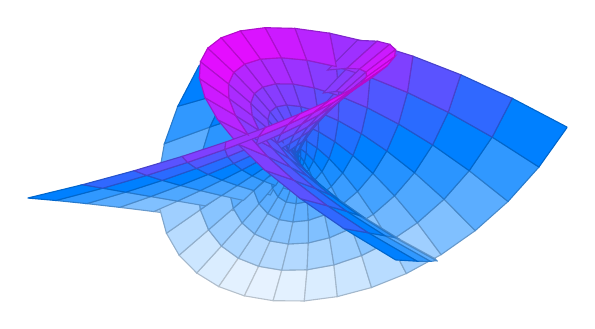
\begin{tikzpicture}
          \begin{axis}[
          hide axis
          ]
             \addplot3[
                 surf,
                 colormap/cool,
                 samples=20,
                 domain=-7:7,
                 y domain=-7:7,
                 z buffer=sort
               ]
               ( {x-x^3/3+x*y^2}, 
                 {-y-x^2*y+y^3/3}, 
                 {x^2-y^2}
               );
          \end{axis}
          
        \end{tikzpicture}
        \caption{Enneper's surface}
        \label{fig: enneper}
    \end{subfigure}
    \caption{Minimal Surfaces}\label{fig: minimal surfaces}
\end{figure}
\end{example}

Lastly, throughout this thesis, we shall employ the folloing notation.
\begin{itemize}
\item $\lambda_{m}$ will denote the $m$-dimensional Lebesgue measure, and we will write $\lambda=\lambda_1$.
\item Given some metric space $(X,d)$, define $B_{r}(x)=\{y \in X \mid d(x,y) \le r\}$. If $X = \R^{m}$ we will sometimes denote the ball by $B_{r}^{m}(x)$ to emphasize the dimension.
\item $\pow{X}$ will denote the power set of $X$.
\item For some open set $U \subseteq \R^n$ let $L^{p}_{loc}(U) = \{f : U \to \R \mid \forall K \subseteq U, K \text{ compact }, |f| \in L^p(K)\}$, i.e. the set functions that are integrable on every compact subsets of its domain
\item If $A$ is a set, $\mathring{A}$ will denote the interior of $A$ and $\overline{A}$ will denote the closure of $A$.
\end{itemize}